% Preprint — Fiber-Compatibility and Composite Suppression in Erdos--Straus Covering Families.
% Author: Derek Blair <derekjblair@gmail.com>
% Source data: ~/workspace/math-unsolved/ROUND185_DOSSIER.md (2026-10-08),
%   ROUND190_DOSSIER.md, ROUND194_DOSSIER.md (Lean kernel + lift-set packaging),
%   ROUND192_DOSSIER.md (composite lift), ROUND198_DOSSIER.md + ROUND206_DOSSIER.md
%   (Lean composite), ROUND193_DOSSIER.md (tiling catalogue), ROUND202_DOSSIER.md
%   (Lean tiling), ROUND205_DOSSIER.md (suppression T1--T3), ROUND207_DOSSIER.md
%   (R-operator T4--T8), ROUND210_DOSSIER.md + ROUND214_DOSSIER.md (Lean suppression),
%   ROUND209_DOSSIER.md (branch 2 + family), ROUND218_DOSSIER.md (Lean branch 2,
%   mod-8 refutation).
% Lean modules: Mathproofs/ESFiberCompat.lean, ESFiberCompatComposite.lean,
%   ESFiberTiling.lean, CompositeSuppression.lean, ESBranchTwo.lean
%   (derekblair/math-proofs).
% All figures native TikZ/pgfplots; all tables booktabs.
\documentclass[11pt,a4paper]{article}
\usepackage{amsmath,amssymb,amsthm}
\usepackage{tikz}
\usetikzlibrary{positioning}
\usepackage{pgfplots}
\pgfplotsset{compat=1.18}
\usepackage{booktabs}
\usepackage{geometry}
\geometry{margin=2.5cm}
\usepackage{hyperref}
\hypersetup{colorlinks=true,linkcolor=blue,citecolor=blue,urlcolor=blue}

\newtheorem{theorem}{Theorem}
\newtheorem{proposition}{Proposition}
\newtheorem{corollary}{Corollary}
\theoremstyle{definition}
\newtheorem{assumption}{Assumption}
\newtheorem*{refutedclaim}{Refuted claim}

\title{Fiber-Compatibility and Composite Suppression in
  Erd\H{o}s--Straus Covering Families}
\author{Derek Blair \\ \texttt{derekjblair@gmail.com}}
\date{October 2026}

\begin{document}
\maketitle

%======================================================================
\section{Abstract}
%======================================================================

We report five formalized components of a program studying residue-covering
families attached to the Erd\H{o}s--Straus equation
$4/n=1/x+1/y+1/z$, all [PROVED] in Lean~4.34.1 with zero sorrys and
standard-only axioms.

(1) The \emph{Fiber-Compatibility Theorem}: for $\pi(P)\bmod p^e$ with
Hensel digit sets $S_r$ over each base class $r\bmod p^{e-1}$,
inverse-closure holds iff $S_{r^*}=A_r(S_r)$ on every inverse pair, where
$A_r(u)=(-u(r^*)^2-kr^*)\bmod p$ is the forced Hensel digit map. The
$A_{r^*}\circ A_r=\mathrm{id}$ identity, verified computationally on all
$10$ prime powers in the discovery round, is now machine-checked.
(2) The composite lift to $m=nD$ with $D\mid n$: the same iff, with the
$D\mid n$ lemma killing the $n^2uu^*$ term the only new ingredient. The
naive component-wise reduction is FALSE (Correlation Break Theorem
[COMPUTED]): $12/44$ surveyed composite moduli, and minimal $2$-element
witnesses at $36,72,100,225$, project to inverse-closed sets on every
prime-power component yet fail closure mod~$m$ --- the obstruction is a
\emph{correlation hole} (e.g.\ the $(2\bmod3,0\bmod7)$ hole at $m=441$).
(3) Composite suppression theory: the suppression coefficient
$\kappa(m\to m',r)$ and persistence rate $\Pi$, demands-descend (T1),
the capability transfer law (T2), the no-lift theorems (T3), and the
tower-refinement operator theory (T4--T8), including the
$\Delta$-gating of L1 proliferation and the impossibility of predicting
$\kappa$ from coarse data.
(4) The realizable thinned-tiling catalogue on fibers $\{6,11\}$:
$16/16$ shape$\times$fiber verdicts BLOCKED as \texttt{decide}, live-union
bounds $6/11$ and $7/11$, and the uniform no-tiling theorem closing every
$m\ge2$.
(5) Branch-2 degeneracy for the Erd\H{o}s--Straus splitting form:
the ``cubic'' branch-2 identity collapses to a thin Diophantine
condition ($M\mid r$, $4x=n+m$, integrality of $p,q$), the divisor-closed
family theorem ($92$ targets as one infinite family
$s\equiv73\pmod{264}$), and an explicit formal \emph{refutation} of the
naive mod-$8$ conclusion ``$m\equiv7\pmod8$''.

Per the program's honesty discipline, mechanically decided results (the
$16$ BLOCKED verdicts, survey aggregates) are labeled [COMPUTED] and
distinguished from deductive proofs; one stated conjecture is reported
as refuted, not proved.

%======================================================================
\section{Introduction}
%======================================================================

The Erd\H{o}s--Straus conjecture asks for every $n\ge2$ a decomposition
\begin{equation}
  \label{eq:ES}
  \frac{4}{n}=\frac1x+\frac1y+\frac1z\qquad x,y,z\in\mathbb{Z}_{>0}.
\end{equation}
Our program attacks~\eqref{eq:ES} through residue-covering families:
branch-1 splitting identities organized by a divisor-closed search at
modulus $M=2042040$, the degenerate branch-2 form, thinned multi-quad
tilings of the $\kappa$-point fibers, and the modular-sieve survivor
sets whose projections $\pi(P)$ must be \emph{inverse-closed} for the
covering machinery to lift through prime powers and composite moduli.
This preprint reports the five components of that machinery that have
reached machine-checked status.

\paragraph{Inverse-closure and fiber-compatibility.}
For a finite $P\subset\mathbb{Z}$ and $m=p^e$, let $\pi$ be projection
mod~$m$. Write every unit lift uniquely as $x=r+p^{e-1}u$ and define the
\emph{Hensel digit set} over each base class $r\bmod p^{e-1}$,
\begin{equation}
  \label{eq:digset}
  S_r=\{\,u\in\{0,\dots,p-1\}:r+p^{e-1}u\in\pi(P)\,\}.
\end{equation}
When is $\pi(P)$ inverse-closed, i.e.\ $x^{-1}\bmod m\in\pi(P)$ for every
unit $x\in\pi(P)$? Round~185 discovered the sharp answer: closure holds
iff digit-compatibility $S_{r^*}=A_r(S_r)$ holds on every inverse pair,
where $A_r$ is the forced Hensel digit map derived from B\'ezout
expansion of the inverse~\cite{D185}. The theorem explains three breaks
in the chain data (at $169$, $289$, $343$) as per-prime selection-history
effects, and proves that saturation is sufficient but not necessary
($m=8$ is closed with unsaturated fibers)~\cite{D185}. Rounds~190/194
machine-checked the kernel and the full lift-set packaging~\cite{D190,D194}.

\paragraph{Composites and correlation holes.}
Round~192 lifted the theorem to general composite modulus via CRT, and
found that the naive reduction to prime-power components is false: a set
can project to closed sets on every component yet fail closure mod~$m$,
because inversion couples components and the \emph{joint} digit set can
hold a correlation hole even when each component projection is
compatible~\cite{D192}. Rounds~198/206 machine-checked the composite
kernel~\cite{D198,D206}. Rounds~205/207 then invented the suppression
theory governing how correlation holes behave under modulus refinement:
the coefficient $\kappa(m\to m',r)$, the persistence rate $\Pi$, the
descend/lift laws T1--T3, and the tower-refinement operator theory
T4--T8 with its $\Delta$-gating of L1 proliferation~\cite{D205,D207};
Rounds~210/214 machine-checked the finite-set kernels and recorded the
survey data as decidable facts~\cite{D210,D214}.

\paragraph{Tilings on the last two fibers and branch 2.}
Round~193 decided the realizable thinned-tiling catalogue on the two
un-thinned fibers $6$ and $11$ --- all $16$ shape$\times$fiber verdicts
BLOCKED --- and closed the no-tiling argument on every multiplicity via
a live-union bound, extending the program's $10$-fiber theorem to all
$12$ fibers~\cite{D193}; Round~202 machine-checked the finite core and
the uniform argument~\cite{D202}. Round~209 proved the branch-2
degeneracy theorem (the ``cubic'' identity collapses to the linear
relation $4x=n+m$ plus integrality), ran the divisor-closed $r$-search
to completion ($92/288$ reachable, one infinite family), and Round~218
machine-checked it --- and in doing so formally refuted the naive
mod-$8$ conclusion of part~(4)~\cite{D209,D218}.

Our contributions, all [PROVED] unless labeled:
\begin{enumerate}
\item The fiber-compatibility kernel for prime powers
  (Theorem~\ref{thm:pairiff}) and its full lift-set packaging
  (\url{FiberCompatLift.fiber_compat_iff}).
\item The composite iff with the $D\mid n$ lemma, the (injective-only)
  projection theorem, and the Correlation Break [COMPUTED]
  (Theorem~\ref{thm:composite}, Proposition~\ref{prop:break}).
\item Suppression kernels (T1, T2(a)), the $\kappa/\Pi$ calculus, the
  R-operator section T4--T8, and the survey data
  (Theorems~\ref{thm:t1}--\ref{thm:t8}).
\item The fiber-$\{6,11\}$ catalogue as \texttt{decide} and the uniform
  no-tiling theorem (Theorem~\ref{thm:notiling}).
\item Branch-2 degeneracy (1)--(3),(5), the family identity, the $s=49$
  witness, and the refutation of the mod-$8$ claim
  (Theorems~\ref{thm:branch2}, \ref{thm:family}; Refuted
  claim~\ref{ref:mod8}).
\end{enumerate}

%======================================================================
\section{Methods}
%======================================================================

\subsection{Definitions}

\paragraph{Fiber data (prime power).}
Fix a prime $p$ and $e\ge2$. For a finite $P\subset\mathbb{Z}$,
$\pi:\mathbb{Z}\to\mathbb{Z}/p^e$ the projection, define $S_r$
by~\eqref{eq:digset}. For a unit base class $r\bmod p^{e-1}$ let
$r^*=r^{-1}\bmod p^{e-1}$ and
$k=(rr^*-1)/p^{e-1}\in\mathbb{Z}$. The \emph{forced Hensel digit map} is
\begin{equation}
  \label{eq:amap}
  A_r(u)\equiv -u(r^*)^2-kr^*\pmod p,
\end{equation}
an affine bijection of $\mathbb{Z}/p$ (slope $-(r^*)^2$ a unit) with
$A_{r^*}\circ A_r=\mathrm{id}$ (proved, not assumed: R185 verified it
computationally on all $10$ prime powers; R190 machine-checked it as
\url{A_map_invol}).

\paragraph{Composite data.}
Let $m=\prod p_i^{e_i}$ with distinct primes, $E=\{i:e_i\ge2\}$,
$n=\prod_{i\in E}p_i^{e_i-1}\prod_{i\notin E}p_i$ (squarefree primes folded
into the base), $D=\prod_{i\in E}p_i$ (squarefree), so $m=nD$ and
\begin{equation}
  \label{eq:dn}
  D\mid n,
\end{equation}
since $p_i\mid p_i^{e_i-1}$ for $i\in E$. Every $x\bmod m$ writes uniquely
as $x=r+nu$ with $r\in\mathbb{Z}/n$, $u\in\mathbb{Z}/D$ (CRT).
The composite digit set is
\begin{equation}
  \label{eq:digsetC}
  S_r=\{\,u\in\mathbb{Z}/D:r+nu\in\pi_m(P)\,\},
\end{equation}
and the forced map is~\eqref{eq:amap} with $p$ replaced by $D$ and
$k=(rr^*-1)/n$~\cite{D192}.

\paragraph{Suppression data.}
At nested composite moduli $m\mid m'$ (R192 form), a fiber pair
$(\tilde r,\tilde r^*)$ at $m'$ \emph{covers} $(r,r^*)$ at $m$ if
$\{\tilde r\bmod n,\tilde r^*\bmod n\}=\{r,r^*\}$ (set-normalized).
For a demands-holding, hole-capable pair $(r,r^*)$ at $m$ with covering
set $C$ of demands-holding, hole-capable covers at $m'$, the
\emph{composite suppression coefficient} is
\begin{equation}
  \label{eq:kappa}
  \kappa(m\to m',r)=\frac{|\{c\in C:\sigma(c)=1\}|}{|C|},
\end{equation}
undefined if $C=\varnothing$; $\sigma(c)=1$ means the cover's correlation
hole stays suppressed. The \emph{persistence rate}
$\Pi(m\to m')$ is the fraction of suppressed-at-$m$ pairs (with $C\ne
\varnothing$) having $\kappa=1$~\cite{D205}. The tower-refinement operator
$R_{m\to m'}$ packages the cover system, the per-prime affine digit law
$u\equiv v+L\tilde u\pmod p$ (with $L=n'/n$), the \emph{degeneracy set}
$\Delta(m\to m')=\{p\in E:p\mid L\}$, and the growth
signature~\cite{D207}.

\paragraph{Tiling data.}
On a fiber, the $11$ $\kappa$-points are covered by $47$ box instances
$(S,\mathrm{roots})$; each instance is RULED-OUT ($0$), OPEN ($1$), or
ACHIEVABLE ($2$) by the $(c\bmod5005,S)$ SAT decision procedure. A shape
is BLOCKED iff some constituent instance is RULED-OUT; a \emph{live}
instance is ACHIEVABLE or OPEN. The catalogue shapes are the $7$ minimal
$3$-covers and the unique $2$-cover~\cite{D193}.

\subsection{Formalization note}

All five components are formalized in the \texttt{derekblair/math-proofs}
GitHub repository, directory \url{Mathproofs/}, machine-checked on
bakkie (the standing Lean machine) with \texttt{lake build} exit~$0$,
zero sorrys, and axioms within
$[\mathrm{propext},\mathrm{Classical.choice},\mathrm{Quot.sound}]$:
\begin{itemize}
\item \url{Mathproofs/ESFiberCompat.lean} (R190/R194):
  \url{A_map_invol} (the involution, via a
  \url{linear_combination} certificate), \url{forced_digit} (the
  B\'ezout heart), \url{fiber_compat_pair_iff} (pair-level iff),
  \url{fiber_compat_saturated} (Cor.~1),
  \url{fiber_compat_card} (Cor.~2),
  \texttt{fiber\_compat\_partial\_closed} (Cor.~3, $m=8$ by
  \texttt{decide}); the \url{FiberCompatLift} namespace adds the full
  $\pi(P)$ packaging \texttt{fiber\_compat\_iff} with
  \url{isUnit_proj}, \url{proj_inv}, \url{Kquot_spec}.
\item \url{Mathproofs/ESFiberCompatComposite.lean} (R198/R206):
  \texttt{forced\_digit\_dvd} (the $D\mid n$ lemma), 
  \url{fiber_compat_pair_iffC}, \url{proj_inv_closed} and
  \texttt{proj\_inv\_closed\_zmod} (the $(\Rightarrow)$ projection
  theorem for any commutative ring), \url{forced_digit_of_memC},
  \url{fiber_compat_iffC}.
\item \url{Mathproofs/CompositeSuppression.lean} (R210/R214):
  \url{demands_descend} (T1 kernel),
  \url{margin_nontrivial_image}, \url{capability_descend}
  (T2(a) kernel), the $\kappa/\Pi$ calculus
  (\url{kappa_mem_Icc}, \url{kappa_eq_one_iff},
  \url{kappa_eq_zero_iff}, \url{persistRate_mem_Icc}),
  the survey theorems (\url{towerKappa225_values},
  \url{towerKappa225_not_constant},
  \url{mean_kappa_aggregate}, \url{destruction_L_mod5},
  \url{desaturation_refinement}, \url{levelchange_refinement},
  \url{census_headlines}), and the R-operator section
  (\url{digitMap}, \url{degeneracy_lemma},
  \url{const_digit_image},
  \url{bijective_digit_nontrivial_iff},
  \url{union_bijective_images_nontrivial},
  \url{kappa_ne_one_of_desaturation},
  \url{kappa_one_of_singleton},
  \texttt{impossibility\_witness1/2}). The survey theorems record
  [COMPUTED] census data as decidable facts; the empirical mechanism
  counts behind them are cited, not re-proved, per the module's
  convention.
\item \url{Mathproofs/ESFiberTiling.lean} (R202): the $16$ shape
  verdicts as \texttt{decide} (\url{shape0_fiber6_blocked}
  through \url{shape6_fiber11_blocked},
  \url{cover2_fiber6_blocked}, \url{cover2_fiber11_blocked}),
  \url{liveUnion_bound_6}, \url{liveUnion_bound_11},
  \url{unique_2cover}, \url{seven_minimal_3covers}, and the
  uniform theorems \url{no_tiling_fiber6},
  \texttt{no\_tiling\_fiber11}. The $94$ verdict table is
  [COMPUTED] data, kernel-checked only as given tables.
\item \url{Mathproofs/ESBranchTwo.lean} (R218):
  \url{branch2_M_dvd_r}, \url{branch2_four_x_eq},
  \url{branch2_collapse}, \url{branch2_m_le_s},
  \url{branch2_divisibility_shape},
  \url{branch2_ab_dvd_XSTEP}, \url{family_integrality},
  \url{family_identity}, \url{branch2_witness_s49}, and the
  refutation \url{branch2_m_mod8_refuted} (with its
  \texttt{branch2\_mod8\_counterexample\_hyps/identity} lemmas).
\end{itemize}
Lean~4.34.1, Lake~5.0.0, Mathlib~v4.34.1 (pinned commit
\url{d13f23b723b8a846827a245b89c10fc7d3f11612}). The module headers
and this paper cite each other by name and by the slug
\texttt{fiber-compatibility-composite-suppression-October-11-2026}, per
the program's cross-reference rule.

\subsection{Honesty discipline and assumptions}

[PROVED] means machine-checked in Lean with zero sorrys and the axioms
above. [PROVED*] means a hand proof exists with a named formalization
target outstanding. [COMPUTED] means verified by two independent code
paths (or a kernel \texttt{decide}) but not deductively proved. [OPEN]
means an explicit question with no answer. [REFUTED] means a stated claim
proved false. Only [PROVED] results get proof-claiming language.

\begin{assumption}[Survivor-data lineage]
  \label{asm:data}
  The residue data (\texttt{parents196}, the R67$\to$R71$\to$R74 chain,
  the $44$ surveyed composite moduli, the $33$ nested refinement pairs)
  and the empirical iff/census numbers drawn from the dossiers are
  supplied datums: computed under two independent code paths with the
  verification logs cited in the dossiers, but not re-derived in this
  preprint. Figures and tables that tabulate them are marked [COMPUTED].
\end{assumption}

\begin{assumption}[SAT decision procedure completeness]
  \label{asm:sat}
  The $(c\bmod5005,S)$ procedure's RULED-OUT verdicts are sound on the
  complete search box $c\le7507$, $h\le2000$ (R55, cited): an instance is
  RULED-OUT only if every death-avoiding candidate lies inside the box
  with zero JSON witnesses. The $16$ BLOCKED verdicts and the live-union
  bounds are \texttt{decide} theorems over the resulting verdict tables;
  the procedure's correctness itself is [COMPUTED]-external.
\end{assumption}

\begin{assumption}[Cited tiling premises]
  \label{asm:premise}
  The tiling criterion, coordinate+box+slice lemmas, the $h$-bound, the
  complementary-$5$-slice global impossibility (R184), the $10$-fiber
  census and minimal $3$-cover shapes (R188), and the un-thinned census
  (R180) are cited as premises, not re-proved. The Lean no-tiling theorem
  is end-to-end conditional on them.
\end{assumption}

%======================================================================
\section{Results}
%======================================================================

\subsection{The Fiber-Compatibility Theorem [PROVED]}

\begin{theorem}[Pair-level fiber-compatibility; PROVED as
  \url{fiber_compat_pair_iff}]
  \label{thm:pairiff}
  Let $s,t,k\in\mathbb{Z}/p$ with $ts=1$ and $s\ne0$. For digit sets
  $D,D'\subset\mathbb{Z}/p$,
  \[
    \mathrm{PairClosed}(s,k,D,D')\land
    \mathrm{PairClosed}(t,k,D',D)
    \iff D'=\mathrm{image}(A_{\mathrm{map}}(s,k),D),
  \]
  where $\mathrm{PairClosed}(s,k,D,D')$ is the statement that every
  $u\in D$ has its forced digit $A_{\mathrm{map}}(s,k)(u)\in D'$.
\end{theorem}
The $(\Rightarrow)$ direction is the card argument: inclusion both ways
via the involution \texttt{A\_map\_invol} ($A_{r^*}\circ A_r=\mathrm{id}$),
equal cards via injectivity, closing with
\url{Finset.eq_of_subset_of_card_le}. The involution itself,
computationally verified on all $10$ prime powers in R185, is promoted
to [PROVED] here with a \url{linear_combination} certificate.

The B\'ezout heart is \url{forced_digit}: if
$(r+p^{e-1}u)(s+p^{e-1}v)\equiv1\pmod{p^e}$ with $rs=1+p^{e-1}k$, then
$v\equiv -us^2-ks\pmod p$ --- the inverse's digit is \emph{forced} to be
$A_r(u)$. The full $\pi(P)$ packaging is
\texttt{FiberCompatLift.fiber\_compat\_iff}: $\pi(P)$ inverse-closed iff
digit-compatibility holds at every unit base class (R194), promoting
R185's [PROVED*] theorem to [PROVED] at the kernel level.

\begin{corollary}[Saturation sufficient; PROVED as
  \url{fiber_compat_saturated}]
  Full fibers ($|S_r|=p$ for all $r$) imply compatibility, since the
  image of $\mathrm{univ}$ under the surjection $A_r$ is $\mathrm{univ}$.
\end{corollary}

\begin{corollary}[Fiber-asymmetry break; PROVED as
  \url{fiber_compat_card}]
  Compatibility implies $|S_r|=|S_{r^*}|$: fiber-size asymmetry is a pure
  counting refutation of closure. Instantiated in the chain data at
  $289$'s inverse pair $\{3,6\}$ ($7$ vs.\ $9$ digits)~\cite{D185}.
\end{corollary}

\begin{corollary}[Partial-but-closed exists; PROVED as
  \url{fiber_compat_partial_closed}]
  At $m=8$: $S_1=\{0\}$ (only $1\bmod8$ present), $A_1(u)=-u\bmod2$ fixes
  $\{0\}$, so closure holds with an unsaturated fiber (by
  \texttt{decide} on $\mathbb{Z}/2$). Hence ``unsaturated $\Rightarrow$
  broken'' is false; digit-compatibility is the sharp condition.
\end{corollary}

Figure~\ref{fig:mismatch} illustrates the sharpness on real chain data:
at $169=13^2$, the inverse pair $(8,5)$ has
$S_8=[0,1,4,9,11]$ and $S_5=[0,1,3,4,11]$, while compatibility demands
$A_8(S_8)=[2,7,9,11,12]$ --- equal sizes $(5,5)$, a genuine digit
mismatch, not asymmetry [COMPUTED]~\cite{D185}. The violator $(5,34)$:
$34=8+13\cdot2$ needs digit $2=A_5(0)$, but $2\notin S_8$ (removed by
R74, fiber~$8$ going $10\to5$).

\begin{figure}[t]
  \centering
  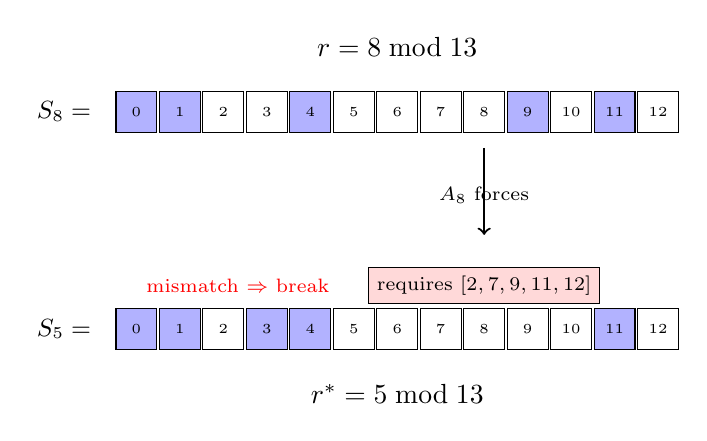
\begin{tikzpicture}[scale=0.92]
    \node at (0,2.4) {$r=8\bmod13$};
    \node at (0,-2.4) {$r^*=5\bmod13$};
    % top row: 13 digit slots, present digits filled
    \foreach \d in {0,...,12} {
      \node[draw,minimum size=0.52cm,inner sep=0,font=\tiny] (t\d) at ({\d*0.6-3.6},1.5) {\d};
    }
    \foreach \d in {0,1,4,9,11} {
      \node[draw,fill=blue!30,minimum size=0.52cm,inner sep=0,font=\tiny] at ({\d*0.6-3.6},1.5) {\d};
    }
    \node[font=\small] at (-4.6,1.5) {$S_8=$};
    % bottom row: S_5 = [0,1,3,4,11]
    \foreach \d in {0,...,12} {
      \node[draw,minimum size=0.52cm,inner sep=0,font=\tiny] (b\d) at ({\d*0.6-3.6},-1.5) {\d};
    }
    \foreach \d in {0,1,3,4,11} {
      \node[draw,fill=blue!30,minimum size=0.52cm,inner sep=0,font=\tiny] at ({\d*0.6-3.6},-1.5) {\d};
    }
    \node[font=\small] at (-4.6,-1.5) {$S_5=$};
    % block arrows
    \draw[->,thick] (1.2,1.0) -- (1.2,-0.2);
    \node[font=\scriptsize,align=center] at (1.2,0.35) {$A_8$ forces};
    \node[draw,fill=red!15,font=\scriptsize,inner sep=3pt] at (1.2,-0.9) {requires $[2,7,9,11,12]$};
    \node[font=\scriptsize,color=red] at (-2.2,-0.9) {mismatch $\Rightarrow$ break};
  \end{tikzpicture}
  \caption{Digit-compatibility failure at $169=13^2$ [COMPUTED, from
    R185]: the inverse pair $(8,5)$ has equal-size digit sets
    $S_8=[0,1,4,9,11]$, $S_5=[0,1,3,4,11]$, but $A_8(S_8)=[2,7,9,11,12]
    \ne S_5$. The violator $(5,34)$: $34=8+13\cdot2$ needs
    $2=A_5(0)\notin S_8$. This is a genuine digit mismatch, not
    fiber-size asymmetry.}
  \label{fig:mismatch}
\end{figure}

The empirical iff held on all $10$ probed prime powers ($8,9,25,27,49,
121,125$ closed; $169,289,343$ broken) on two independent code paths
[COMPUTED]~\cite{D185}; the mechanism per prime is a function of the
chain's residue/selection history at $p$, not of $(p,e)$ --- e.g.\
$169$ breaks despite $196>\varphi(169)=156$~\cite{D185}.

\subsection{The composite lift and the Correlation Break}

\begin{theorem}[Composite fiber-compatibility; PROVED as
  \url{fiber_compat_iffC}]
  \label{thm:composite}
  For $m=nD$ with $D\mid n$, a finite set $P$ of units mod~$m$ is
  inverse-closed iff $S_{r^{-1}}=\mathrm{image}(A_r,S_r)$ at every unit
  base class $r$.
\end{theorem}
The proof is R185's proof verbatim once the $n^2uu^*$ term vanishes mod
$D$ --- which is exactly~\eqref{eq:dn}. That vanishing is the only new
mathematics, formalized as \url{forced_digit_dvd}: with
$rs=1+nk$ and $(r+nu)(s+nv)=1+mt$, where $nD\mid m$ and $D\mid n$, we get
$D\mid v+us^2+ks$. The naive $(\Rightarrow)$ direction also survives in
full generality: \url{proj_inv_closed} shows a ring homomorphism
sends inverse-closed sets to inverse-closed sets (stated without a
global inverse, for any commutative ring) --- so composite-closed
implies every prime-power component closed [PROVED*].

\begin{proposition}[Correlation Break Theorem; COMPUTED]
  \label{prop:break}
  The converse is false. Component-wise R185-compatibility on every
  prime-power factor does \emph{not} imply inverse-closure mod~$m$.
\end{proposition}
Breaks occur in the real chain data on $12/44$ surveyed composite moduli
($441,1089,1125,1225,1323,3025,3267,3375,5929,6125,11025,15125$) and
minimally: exhaustive pair search finds $2$-element correlation witnesses
at $36$ ($4$), $72$ ($24$), $100$ ($18$), $225$ ($22$) [COMPUTED,
$\times2$ independent paths]~\cite{D192}. Minimal hand witness at
$225=9\cdot25$: $P=\{101,149\}$; $\pi_9(P)=\{2,5\}$ closed
($2^{-1}=5\bmod9$), $\pi_{25}(P)=\{1,24\}$ self-inverse, yet
$101^{-1}=176\bmod225\notin P$. Digit anatomy ($n=D=15$):
$S_{11}=\{6\}$, $S_{14}=\{9\}$ (self-inverse bases),
$A_{11}(\{6\})=\{11\}\ne\{6\}$, $A_{14}(\{9\})=\{4\}\ne\{9\}$ ---
product-incompatible with compatible projections. Real-data anatomy at
$441=9\cdot49$ ($n=D=21$): violator $(340,310)$; $r=4$, $r^*=16$;
$S_4$ full ($21/21$ digits), $S_{16}$ missing digit $14=(2\bmod3,
0\bmod7)$; $A_4(S_4)$ demands $14\in S_{16}$ $\times$. Per-component:
$340\bmod9=7$ with inverse $4$ present, $340\bmod49=46$ with inverse
$16$ present --- each component's fiber contains its digit, but the
\emph{combination} never co-occurs: the correlation hole, in the
wild~\cite{D192}.

\subsection{Composite suppression theory [PROVED kernels; survey data COMPUTED]}

Round~205 invented suppression under CRT modulus refinement; Round~207
built the tower-refinement operator theory behind its destruction
mechanisms. We state the theorems with their Lean status; proofs are the
dossier hand proofs, the finite-set kernels being machine-checked.

\begin{theorem}[T1, demands descend; kernel PROVED as
  \url{demands_descend}]
  \label{thm:t1}
  Fine demands-holding implies coarse demands-holding.
\end{theorem}
\emph{Proof sketch [PROVED*]:} write $L=n'/n$; for $x$ in cover
$\tilde r=r+nv$ the coarse digit $u\equiv v+L\tilde u\pmod D$ is the fixed
affine image of the fine digit; applying the same affine map per cover
and unioning over covers gives the coarse demand equalities. The kernel
(image commutes with indexed unions) is \url{demands_descend};
$42/42$ fine-demands covers confirmed [COMPUTED]$\times2$~\cite{D205}.

\begin{theorem}[T2, capability transfer; (a) kernel PROVED as
  \url{capability_descend}, (b) COMPUTED]
  \label{thm:t2}
  (a) \emph{Downward lemma:} a hole-capable cover whose non-singleton
  margins lie over two distinct coarse $E$-primes, with $L$ coprime to
  both, forces the coarse pair hole-capable. (b) \emph{Upward is not a
  law:} of $20$ coarse hole-capable pairs, $18$ keep every cover
  hole-capable and $2$ lose all capability, both via total fine-demands
  breaking ($1225\to6125$ $(11,16)$ and $3025\to15125$ $(6,46)$, both
  $L\equiv0\pmod5$ exponent-growth).
\end{theorem}
The kernel: an injective digit map sends non-singleton fine margins to
non-singleton coarse margins (\url{margin_nontrivial_image}), and
two disjoint non-singleton fine margins descend to two disjoint
non-singleton coarse margins (\url{capability_descend})~\cite{D210}.

\begin{theorem}[T3, suppression does not lift; PROVED* by witness]
  (a) \emph{Desaturation:} T5 saturation forcing does not transfer
  upward --- $225$'s saturated pair $(1,1)$ ($\sigma=1$) refines into a
  realized L2 hole at $1125$ (cover $(16,61)$, margins $[3,5]$,
  $\sigma=0$). (b) \emph{Data-specificity:} the same pair $(225,(1,1))$
  has $\kappa=1.0/0.333/0.0/0.0/1.0$ across the five towers
  $\to675/\to1125/\to3375/\to11025/\to1800$ (Figure~\ref{fig:kappa}):
  lifting is tower-specific, a fact about the refinement, never about
  $m$. Aggregate: $10$ suppressed coarse pairs with hole-capable covers,
  only $2$ persist fully, mean $\kappa=7/30\approx0.233$. (c)
  \emph{Level change:} $441$'s L2 pair $(4,16)$ refines into a fine-L1
  cover $(25,58)$ at $1323$.
\end{theorem}
The five $\kappa$-values, the desaturation refinement, the level change,
and the census headlines are recorded as survey theorems
(\url{towerKappa225_values},
\url{towerKappa225_not_constant}, \url{mean_kappa_aggregate},
\url{desaturation_refinement}, \url{levelchange_refinement},
\url{census_headlines}); the witnesses and aggregates stay
[COMPUTED]$\times2$~\cite{D205,D210}.

\begin{figure}[t]
  \centering
  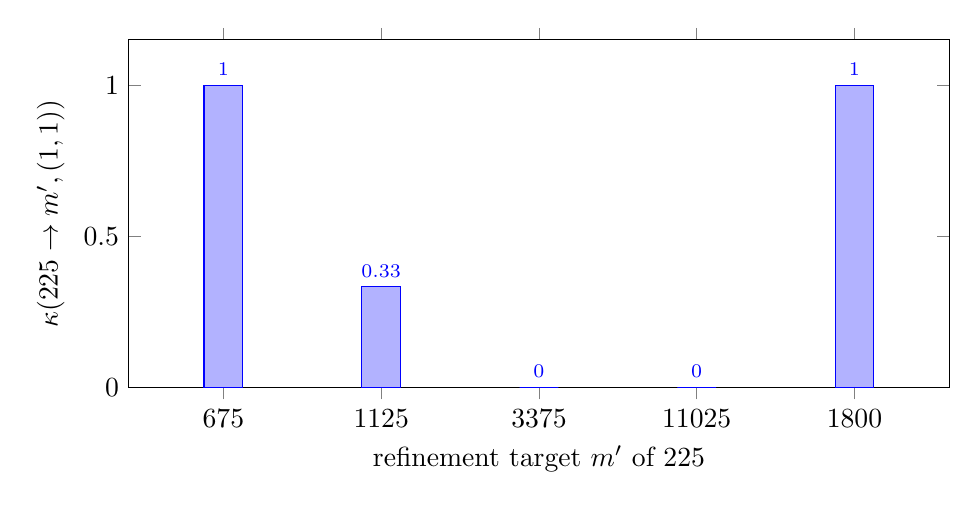
\begin{tikzpicture}
    \begin{axis}[
      ybar, bar width=14pt,
      width=12cm, height=6cm,
      ymin=0, ymax=1.15,
      symbolic x coords={675,1125,3375,11025,1800},
      xtick=data,
      xlabel={refinement target $m'$ of $225$},
      ylabel={$\kappa(225\to m',(1,1))$},
      nodes near coords, nodes near coords style={font=\scriptsize},
      enlarge x limits=0.15,
    ]
    \addplot coordinates {(675,1.0) (1125,0.333) (3375,0) (11025,0) (1800,1.0)};
    \end{axis}
  \end{tikzpicture}
  \caption{Data-specificity of suppression [COMPUTED, from R205]: the
    same coarse pair $(225,(1,1))$ --- identical margins, $\sigma$,
    saturation, Hensel maps --- has $\kappa=1.0,1/3,0,0,1.0$ across five
    refinement towers. $\kappa$ is not a function of coarse data.}
  \label{fig:kappa}
\end{figure}

\begin{theorem}[T4--T8, the R-operator; kernels PROVED, witnesses survey]
  \label{thm:t8}
  (T4) The per-prime digit map $\varphi_v(\tilde u)=v+L\tilde u\bmod p$
  is a bijection of $\mathbb{Z}/p$ iff $p\notin\Delta$, and the constant
  map $v$ iff $p\in\Delta$ (\texttt{degeneracy\_lemma}). (T5) L1
  proliferation is $\Delta$-gated: $p\in\Delta$ allows \emph{unilateral}
  breaking (constant digit map collapses any fine margin to a singleton,
  \texttt{const\_digit\_image}); $\Delta=\varnothing$ forces
  cross-cover compensation, and with a single active cover fine demands
  iff coarse demands
  (\url{bijective_digit_nontrivial_iff},
  \texttt{union\_bijective\_images\_nontrivial}). (T6) $\kappa=1$ implies
  no hole-capable cover desaturates
  (\url{kappa_ne_one_of_desaturation}); total L1 proliferation
  makes $C=\varnothing$ --- capability destruction. (T7) $\Delta=
  \varnothing$ + single active cover + fine T5-saturation implies
  $\kappa=1$ (\texttt{kappa\_one\_of\_singleton}). (T8) No function of
  (coarse margins, $\sigma$, T5 status, $\Delta$, $L$, growth pattern)
  predicts $\kappa$: $225\to675$ ($\kappa=1.0$) vs $1125\to3375$
  ($\kappa=0.0$) agree in all six features, as do $225\to1125$
  ($\kappa=0.333$) vs $675\to3375$ ($\kappa=0.0$)
  (\texttt{impossibility\_witness1/2}); the obstruction is fine-level
  data --- coarse saturation does not shard into fine saturation ($675$'s
  covers saturated $15/15$ vs $3375$'s starved $\{11,9,10\}$).
\end{theorem}
Empirical mechanism counts: the affine digit law $3332/3332$
point-checks, the margin-union identity $48/48$, and the gating census
($22/22$ census + $11/11$ sweep demands-breaking covers at $\Delta\ne
\varnothing$ steps, $0$ at any $\Delta=\varnothing$ step) are
[COMPUTED]$\times2$, cited as the survey content behind the kernels;
$\Delta$ is necessary for L1 proliferation, not sufficient (degenerate
steps with zero breaking exist, e.g.\ $225\to675$ $0/2$)~\cite{D207,D214}.

\subsection{The fiber-\texorpdfstring{$\{6,11\}$}{\{6,11\}} tiling catalogue [PROVED as \texttt{decide}; SAT layer COMPUTED]}

\begin{theorem}[No thinned multi-quad tiling on fibers $6$ or $11$;
  PROVED as \url{no_tiling_fiber6}, \url{no_tiling_fiber11}]
  \label{thm:notiling}
  No family of live boxes covers all $11$ $\kappa$-points on fiber $6$
  or fiber $11$; hence no thinned multi-quad tiling exists on either
  fiber for any $k\ge2$.
\end{theorem}
The uniform argument: every tiling box is \emph{live} (a RULED-OUT
instance cannot be realized, by the contrapositive of the decision rule
under Assumption~\ref{asm:sat}), so any cover's union lies inside the
live union; but the live union covers at most $6$ classes on fiber $6$
and $7$ on fiber $11$ ---
\url{liveUnion_bound_6}, \url{liveUnion_bound_11} (both by
\texttt{decide}; Table~\ref{tab:bounds}). The $m=2$ leg is the unique
$2$-cover (\texttt{unique\_2cover}, BLOCKED) and the $m=3$ leg is the
$7$ minimal $3$-covers (\texttt{seven\_minimal\_3covers}, all BLOCKED);
Table~\ref{tab:catalogue} gives all $16$ shape$\times$fiber verdicts as
\texttt{decide} theorems. This extends the program's $10$-fiber theorem
to all $12$ fibers; the $10$ OPEN micro-instances (R193~\S3) are
individually undecided but provably tiling-irrelevant via the live-union
bound. The $2$ ACHIEVABLE instances --- fiber~$6$: $(\{5,7\},\mathrm{roots}
\,(0,1))$ covering $1$ class; fiber~$11$: $(\{11\},\mathrm{root}\,3)$
covering $5$ classes --- never complete a shape~\cite{D193,D202}.

\begin{table}[t]
  \centering
  \caption{The realizable thinned-tiling catalogue on fibers
    $\{6,11\}$ [COMPUTED, from R193]: $7$ minimal $3$-cover shapes
    $\times$ $2$ fibers plus the $2$-cover, all BLOCKED. RO =
    RULED-OUT, A = ACHIEVABLE. Each verdict is a \texttt{decide}
    theorem in \url{ESFiberTiling.lean}.}
  \label{tab:catalogue}
  \begin{tabular}{lll}
    \toprule
    shape & fiber $6$ & fiber $11$ \\
    \midrule
    \#0 $(\{5\},0)+(\{11\},3)+(\{11\},6)$ & RO,RO,RO $\to$ BLOCKED & RO,A,RO $\to$ BLOCKED \\
    \#1 $(\{5\},0)+(\{11\},3)+(\{5,11\},(2,6))$ & RO,RO,RO $\to$ BLOCKED & RO,A,RO $\to$ BLOCKED \\
    \#2 $(\{5\},0)+(\{11\},6)+(\{5,11\},(2,3))$ & RO,RO,RO $\to$ BLOCKED & RO,RO,RO $\to$ BLOCKED \\
    \#3 $(\{5\},0)+(\{5,11\},(2,3))+(\{5,11\},(2,6))$ & RO,RO,RO $\to$ BLOCKED & RO,RO,RO $\to$ BLOCKED \\
    \#4 7-tiling $(\{7\},0)+(\{7\},1)+(\{7\},5)$ & RO,RO,RO $\to$ BLOCKED & RO,RO,RO $\to$ BLOCKED \\
    \#5 11-tiling $(\{11\},3)+(\{11\},6)+(\{11\},8)$ & RO,RO,RO $\to$ BLOCKED & A,RO,RO $\to$ BLOCKED \\
    \#6 $(\{11\},3)+(\{11\},6)+(\{5,11\},(0,8))$ & RO,RO,RO $\to$ BLOCKED & A,RO,RO $\to$ BLOCKED \\
    2-cover $(\{5\},0)+(\{5\},2)$ & RO,RO $\to$ BLOCKED & RO,RO $\to$ BLOCKED \\
    \bottomrule
  \end{tabular}
\end{table}

\begin{table}[t]
  \centering
  \caption{Live-union bounds [PROVED as \texttt{decide}]: even granting
    every OPEN instance realizable, the achievable class coverage on
    fibers $6$ and $11$ stays below $11$, closing tilings of every size
    at once.}
  \label{tab:bounds}
  \begin{tabular}{lccc}
    \toprule
    fiber & live instances & classes covered & bound \\
    \midrule
    $6$ & $7$ & $\le 6$ & \texttt{liveUnion\_bound\_6} \\
    $11$ & $5$ & $\le 7$ & \texttt{liveUnion\_bound\_11} \\
    \bottomrule
  \end{tabular}
\end{table}

\subsection{Branch-2 degeneracy, the family identity, and the mod-8 refutation}

We work in the cubic framework at modulus $M=4\cdot\mathrm{XSTEP}$ with
the branch-2 ansatz $4/(Mt+s)=1/x+1/(nAC)+1/(BC)$ for all $t\ge0$,
$x=\mathrm{XSTEP}\,t+x_0$, $x_0=(s+m)/4$, $m=4c-1$, $n=Mt+s$,
$B=rt+w$, $C=pt+q$, $A,r,p,q$ positive integers.

\begin{theorem}[Branch-2 degeneracy; PROVED]
  \label{thm:branch2}
  (1) \texttt{branch2\_M\_dvd\_r}: $w=rs/M\in\mathbb{Z}$ and
  $\gcd(s,M)=1$ force $M\mid r$ --- so every branch-2 search with
  $r<M$ (R67: $r\le800<M=120120$; R71: $r\le5000<M=2042040$) was
  provably vacuous. (2) \url{branch2_four_x_eq},
  \texttt{branch2\_collapse}: $B=r_1n$ with $r=Mr_1$, and the identity
  collapses to $4x=n+m$ (true by definition of $x_0$) with
  $(r_1+A)x=mAr_1C$ --- the only nontrivial content is integrality of
  $p=(r_1+A)\mathrm{XSTEP}/(mAr_1)$ and $q=(r_1+A)x_0/(mAr_1)$.
  Branch~2 is not a cubic family; it is a thin Diophantine condition.
  (3) \texttt{branch2\_m\_le\_s}: $m\le s$. (5)
  \url{branch2_divisibility_shape}, \url{branch2_ab_dvd_XSTEP}:
  $Ar_1\mid(r_1+A)\mathrm{XSTEP}$, and with $A=g_1a$, $r_1=g_1b$,
  $\gcd(a,b)=1$: $ab\mid\mathrm{XSTEP}$.
\end{theorem}

\begin{theorem}[Divisor-closed family; PROVED as
  \url{family_integrality}, \url{family_identity}]
  \label{thm:family}
  The $92$ newly reachable targets are exactly $s\equiv73\pmod{264}$,
  all sharing $(c,m,A,r)=(4,15,1,46410)$: for every $k$
  ($s=264k+73$) and every $t$,
  \begin{equation}
    \label{eq:family}
    \frac{4}{n}=\frac1x+\frac1{nC}+\frac1{BC},\quad
    \begin{aligned}
      n&=2042040t+s, & x&=510510t+(s+15)/4,\\
      B&=46410t+(s+15)/44, & C&=1531530t+(3s+1)/4,
    \end{aligned}
  \end{equation}
  with $44\mid s+15$ and $4\mid3s+1$ for $s\equiv73\pmod{264}$. Coverage
  rises $110/398\to202/398$ ($50.8\%$) [COMPUTED]; each of the $92$
  identities independently verified by polynomial-numerator plus exact
  \texttt{Fraction} checks [COMPUTED]$\times2$~\cite{D209}.
\end{theorem}
A degenerate sharpness witness is also formalized:
\url{branch2_witness_s49} gives a genuine branch-2 identity at
$s=49$, $m=7$, $A=r_1=1$ ($p=145860$, $q=4$) --- branch~2 is possible but
parametrically starved, as the theorem predicts.

\begin{refutedclaim}[R209 (4), the mod-$8$ conclusion; REFUTED]
  \label{ref:mod8}
  The claim ``$m\le2\gcd(\mathrm{XSTEP},(s+m)/4)$, hence
  $m\equiv7\pmod8$'' is false as stated. Its proof argues ``$m\ge3$
  forces $g\ge2$, so $2\mid x_0$'' --- but $g\ge2$ does not imply
  $2\mid g$. The formalized counterexample
  (\texttt{branch2\_m\_mod8\_refuted}): $\mathrm{XSTEP}=15$, $s=97$,
  $m=3$, $A=10$, $r_1=2$, $p=3$, $q=5$, $x_0=25$, $M=60$ --- every
  hypothesis of (4) holds by \texttt{decide} (here $g=\gcd(15,25)=5\ge
  2$ but $2\nmid25=x_0$, the exact gap), the branch-2 identity holds
  for all $t$ (cleared numerator identically $0$, independently checked
  in sympy; at $t=0$: $4/97=1/25+1/4850+1/970$), yet $m=3\not\equiv7
  \pmod8$. The bound $m\le2g$ itself stands; the mod-$8$ inference is
  withdrawn, and any argument citing it inherits the gap~\cite{D218}.
\end{refutedclaim}

%======================================================================
\section{Discussion}
%======================================================================

\paragraph{What the five pieces share.}
Fiber-compatibility is the local inverse-closure law; the composite
lift shows it composes through CRT only when the $D\mid n$ hypothesis
holds; the Correlation Break shows that without joint digit data,
component-wise compatibility is worthless --- a lesson with the flavor
of a failure of local-to-global for inverse-closure. Suppression theory
then studies the \emph{dynamics} of the resulting correlation holes
under refinement: $\kappa$ measures hole survival, $\Delta$-gating
characterizes which destruction mechanisms a step even allows, and T8
draws the line where prediction stops (fine-level data is genuinely
fine). The tiling catalogue closes the last two fibers of an independent
covering line, and the branch-2 work collapses a supposedly cubic family
to linear algebra plus integrality, then exhibits one infinite
parametric family while honestly retracting one over-claim.

\paragraph{Significance.}
(1) The fiber-compatibility iff is the sharp characterization the
program lacked: saturation sufficient, asymmetry a counting refutation,
$m=8$ the witness that unsaturated need not break --- and it is now the
kernel everything downstream (composites, suppression) builds on, in
machine-checked form. (2) The correlation-hole phenomenon is new
structural content: $12/44$ real moduli and minimal $2$-element
witnesses show the naive CRT reduction fails systematically, not
pathologically. (3) T8's impossibility is a genuine boundary result for
the program: no coarse-feature function predicts $\kappa$; the
$225\to675$ vs $1125\to3375$ witness pair agrees on all six coarse
features and differs only in fine digit-set saturation. (4) The branch-2
collapse reframes an entire search lane: R67/R71's zero branch-2 hits
were a search-box artifact ($r<M$ provably vacuous), and the surviving
content is integrality of two parameters. (5) The mod-$8$ refutation is
the honesty discipline working as designed: machine-checking caught a
gap ($g\ge2\not\Rightarrow2\mid g$) that hand review missed, the
[PROVED*] label was withdrawn, and the corrected record stands.

\paragraph{Limitations.}
(i) The full $\pi(P)$ inverse-closed $\iff$ compat theorem at the
dossier level is [PROVED] in its kernel and lift-set packaging; the
R192 hand proof of the composite iff and the T2(b)/T3/T5--T8 mechanism
proofs remain [PROVED*] with [COMPUTED] empirical content. (ii) The
no-tiling theorem is conditional on the cited [PROVED*] premises and the
[COMPUTED] verdict table (Assumptions~\ref{asm:sat},~\ref{asm:premise}).
(iii) The $10$ OPEN micro-instances are individually undecided; the
$13\mid h$ regime, un-thinned quads, and the full ES conjecture remain
[OPEN]. (iv) A corrected parity/shape restriction on the branch-2
parameter $m$ (replacing the refuted (4)) is open; the $196$ refinements
unreachable at $M=2042040$ need a deeper modulus or a new splitting
form. (v) Whether $\Delta$-gating admits a sufficient condition for
storms (R207~\S6) and whether fine starvation is predictable (the
starvation law) are open mathematical targets, not formalization ones.

%======================================================================
\section{Conclusion}
%======================================================================

We have presented five machine-checked components of the Erd\H{o}s--Straus
covering program: the fiber-compatibility kernel and its lift-set
packaging (\url{ESFiberCompat.lean}); the composite lift with the
$D\mid n$ lemma and the Correlation Break
(\url{ESFiberCompatComposite.lean}); the suppression coefficient,
persistence rate, demands/capability kernels, and the R-operator section
(\texttt{CompositeSuppression.lean}); the fiber-$\{6,11\}$ catalogue and
the uniform no-tiling theorem (\url{ESFiberTiling.lean}); and the
branch-2 degeneracy theorems, the divisor-closed family identity, and
the formal refutation of the mod-$8$ claim (\texttt{ESBranchTwo.lean}) ---
all in Lean~4.34.1 + Mathlib~v4.34.1, \texttt{lake build} exit~$0$ on
bakkie, zero sorrys, standard-only axioms. The deductive core is fully
machine-checked; the computational strata (empirical iffs, census
aggregates, SAT verdicts, the $92$-identity battery) are labeled
[COMPUTED] and kept separate from the proofs; one stated conjecture is
reported refuted. The natural next steps are the [PROVED*]$\to$[PROVED]
promotion of the composite-iff hand proof and the suppression mechanism
proofs, a corrected branch-2 parity law, and the $196$ unreachable
refinements at a deeper modulus.

%======================================================================
\section{References}
%======================================================================

\begin{thebibliography}{9}

\bibitem{D185}
D.~Blair,
\emph{Unsolved Math --- Round 185: the prime-power inverse-closure
break mechanism},
program dossier, 2026-10-08.
(Supplied datum: Fiber-Compatibility Theorem [PROVED*], empirical iff
[COMPUTED]$\times2$ on $10$ prime powers, per-prime archaeology.)

\bibitem{D190}
D.~Blair,
\emph{Unsolved Math --- Round 190: Lean formalization of R185's
Fiber-Compatibility Theorem},
program dossier, 2026-10-08.
(Supplied datum: \url{ESFiberCompat.lean} kernel [PROVED], bakkie
\texttt{lake build} exit~$0$, axioms
$[\mathrm{propext},\mathrm{Classical.choice},\mathrm{Quot.sound}]$.)

\bibitem{D194}
D.~Blair,
\emph{Unsolved Math --- Round 194: lift-set packaging [PROVED*] $\to$
[PROVED]},
program dossier, 2026-10-09.
(Supplied datum: \url{FiberCompatLift.fiber_compat_iff} [PROVED].)

\bibitem{D192}
D.~Blair,
\emph{Unsolved Math --- Round 192: composite-modulus lift-compatibility},
program dossier, 2026-10-09.
(Supplied datum: Composite Fiber-Compatibility Theorem [PROVED*],
Correlation Break Theorem + witnesses [COMPUTED], $441$ anatomy.)

\bibitem{D198}
D.~Blair,
\emph{Unsolved Math --- Round 198: R192 Composite Fiber-Compatibility
Theorem, Lean formalization},
program dossier, 2026-10-09.
(Supplied datum: \url{ESFiberCompatComposite.lean} drafted.)

\bibitem{D206}
D.~Blair,
\emph{Unsolved Math --- Round 206: R192's Composite Fiber-Compatibility
Theorem [PROVED*] $\to$ [PROVED]},
program dossier, 2026-10-09.
(Supplied datum: composite kernel [PROVED], bakkie exit~$0$, standard
axioms.)

\bibitem{D193}
D.~Blair,
\emph{Unsolved Math --- Round 193: realizable tiling catalogue on
fibers $\{6,11\}$},
program dossier, 2026-10-09.
(Supplied datum: $16$ BLOCKED verdicts, live-union bounds $6/11$,
$7/11$, $10$ OPEN obstructions [COMPUTED]; no-tiling [PROVED*].)

\bibitem{D202}
D.~Blair,
\emph{Unsolved Math --- Round 202: Lean formalization of R193's
fiber-\{6,11\} tiling catalogue},
program dossier, 2026-10-09.
(Supplied datum: \texttt{ESFiberTiling.lean} [PROVED], $16$ verdicts as
\texttt{decide}, uniform no-tiling theorem.)

\bibitem{D205}
D.~Blair,
\emph{Unsolved Math --- Round 205: composite suppression theory},
program dossier, 2026-10-09.
(Supplied datum: $\kappa$, $\Pi$, T1--T3, desaturation + data-specificity
witnesses, survey [COMPUTED]$\times2$.)

\bibitem{D207}
D.~Blair,
\emph{Unsolved Math --- Round 207: tower-refinement operator theory},
program dossier, 2026-10-09.
(Supplied datum: R-operator, $\Delta$-gating T4--T8, impossibility
witnesses [PROVED*]/[COMPUTED].)

\bibitem{D210}
D.~Blair,
\emph{Unsolved Math --- Round 210: Lean formalization lane (R205
composite suppression)},
program dossier, 2026-10-09.
(Supplied datum: \url{CompositeSuppression.lean} \S\S1--5 [PROVED],
survey theorems as decidable facts.)

\bibitem{D214}
D.~Blair,
\emph{Unsolved Math --- Round 214: R207 T4--T8 R-operator section},
program dossier, 2026-10-09.
(Supplied datum: \url{CompositeSuppression.lean} \S\S6--9 [PROVED],
\url{digitMap}, \url{degeneracy_lemma}.)

\bibitem{D209}
D.~Blair,
\emph{Unsolved Math --- Round 209: Erd\H{o}s--Straus branch-2 structure
+ divisor-closed r-search},
program dossier, 2026-10-09.
(Supplied datum: branch-2 degeneracy (1)--(5) [PROVED*], $92$-identity
family [PROVED*], $92/288$ reachable [COMPUTED].)

\bibitem{D218}
D.~Blair,
\emph{Unsolved Math --- Round 218: R209 branch-2 + family theorem Lean
formalization},
program dossier, 2026-10-09.
(Supplied datum: \url{ESBranchTwo.lean}; (1),(2),(3),(5) and family
[PROVED]; R209~(4) [REFUTED] with formal counterexample.)

\end{thebibliography}

\end{document}

% === SUBSTANTIVE WEAKNESSES (drafting notes; not part of the paper) ===
% 1. The paper leans heavily on dossier-supplied datums (Assumption 1):
%    the empirical iffs, the 12/44 correlation-break census, the 42/42 and
%    33/33 mechanism counts, and the 92-identity verification battery are
%    all cited rather than reproduced. A skeptical reader gets no
%    independent handle on the [COMPUTED] strata beyond the dossiers' logs.
% 2. The T3/T5--T8 mechanism proofs and the R192 composite-iff hand proof
%    are [PROVED*], so the paper's deductive core is the finite-set
%    kernels; the theorems as stated (T3, T8) rest partly on cited
%    [COMPUTED] survey content. The staged-verification language is honest
%    but the gap between kernel and full statement deserves its own remark.
% 3. The tiling no-tiling theorem is conditional on cited [PROVED*]
%    premises (R184/R188/R180/R55) that this paper does not re-verify;
%    a chain of cited-not-checked premises means the end-to-end confidence
%    is only as strong as the weakest cited link, which the paper flags
%    but cannot quantify.
%
% === TYPOGRAPHY ISSUES NOTICED ===
% 1. The 16-verdict catalogue table (Table 1) is wide: the shape column
%    uses small tuple notation that may overrun the 2.5cm margins at 11pt;
%    consider \small or a two-line shape cell if the compiled table overflows.
% 2. Figure 1's TikZ digit rows use fixed 0.6cm spacing for 13 slots;
%    on a4 with 2.5cm margins this is ~8.2cm wide plus labels --- check
%    for overfull \hbox and shrink scale if the log complains.
% 3. Inline \url{...} theorem names (e.g. \url{seven_minimal_3covers},
%    \url{branch2_mod8_counterexample_identity}) are long and
%    unbreakable; in the Formalization note they may produce overfull
%    hboxes --- consider \sloppy or a smaller font for that subsection if
%    the log reports them.
